\documentclass[tikz]{standalone}
% \usepackage{tikz} % already loaded by the documentclass


\begin{document}
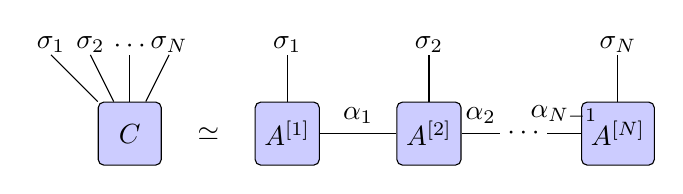
\begin{tikzpicture}[
    core/.style={draw,fill=blue!20,rounded corners=2pt,minimum size=8mm},
    phyleg/.style={-},
    bond/.style={-},
  ]
  \node[core] (C) at (-2,0) {$C$};
  \draw[bond] (C) -- (-3,1) node[above, yshift=-1mm]{$\sigma_1$};
  \draw[bond] (C) -- (-2.5,1) node[above, yshift=-1mm]{$\sigma_2$};
  \draw[bond] (C) -- (-2.0,1) node[above, yshift=-1mm]{$\cdots$};
  \draw[bond] (C) -- (-1.5,1) node[above, yshift=-1mm]{$\sigma_N$};
  \node at (-1,0) {$\simeq$};
  \node[core] (A1) at (0,0) {$A^{[1]}$};
  \node[core] (A2) at (1.8,0) {$A^{[2]}$};
  \node at (3.0,0) {$\cdots$};
  \node[core] (AN) at (4.2,0) {$A^{[N]}$};
  \draw[bond] (A1.east) -- (A2.west) node[midway,above]{$\alpha_1$};
  \draw[bond] (A2.east) -- (2.7,0) node[midway,above]{$\alpha_2$};
  \draw[bond] (3.3,0) -- (AN.west) node[midway,above]{$\alpha_{N-1}$};
  \foreach \i/\x in {1/0,2/1.8,N/4.2}{
      \draw[phyleg] (\x,0.4) -- ++(0,0.6) node[above, yshift=-1mm] {$\sigma_\i$};
    }
\end{tikzpicture}
\end{document}
      